\documentclass[12pt]{article}
\usepackage{times} 			% use Times New Roman font

\usepackage[margin=1in]{geometry}   % sets 1 inch margins on all sides
\usepackage{hyperref}               % for URL formatting
\usepackage[pdftex]{graphicx}       % So includegraphics will work
\setlength{\parskip}{1em}           % skip 1em between paragraphs
\usepackage{indentfirst}            % indent the first line of each paragraph
\usepackage{datetime}
\usepackage[small, bf]{caption}
\usepackage{listings}               % for code listings
\usepackage{xcolor}                 % for styling code
\usepackage{multirow}

%New colors defined below
\definecolor{backcolour}{RGB}{246, 246, 246}   % 0xF6, 0xF6, 0xF6
\definecolor{codegreen}{RGB}{16, 124, 2}       % 0x10, 0x7C, 0x02
\definecolor{codepurple}{RGB}{170, 0, 217}     % 0xAA, 0x00, 0xD9
\definecolor{codered}{RGB}{154, 0, 18}         % 0x9A, 0x00, 0x12

%Code listing style named "gcolabstyle" - matches Google Colab
\lstdefinestyle{gcolabstyle}{
  basicstyle=\ttfamily\small,
  backgroundcolor=\color{backcolour},   
  commentstyle=\itshape\color{codegreen},
  keywordstyle=\color{codepurple},
  stringstyle=\color{codered},
  numberstyle=\ttfamily\footnotesize\color{darkgray}, 
  breakatwhitespace=false,         
  breaklines=true,                 
  captionpos=b,                    
  keepspaces=true,                 
  numbers=left,                    
  numbersep=5pt,                  
  showspaces=false,                
  showstringspaces=false,
  showtabs=false,                  
  tabsize=2
}

\lstset{style=gcolabstyle}      %set gcolabstyle code listing

% for long tables
\usepackage[utf8]{inputenc}
\usepackage{longtable}

% to make long URIs break nicely
\makeatletter
\g@addto@macro{\UrlBreaks}{\UrlOrds}
\makeatother

% for fancy page headings
\usepackage{fancyhdr}
\setlength{\headheight}{13.6pt} % to remove fancyhdr warning
\pagestyle{fancy}
\fancyhf{}
\rhead{\small \thepage}
\lhead{\small HW3, WELLS}
\chead{\small CS 532, Spring 2021} 

%-------------------------------------------------------------------------
\begin{document}

\begin{centering}
{\large\textbf{HW3 - RANKING WEBPAGES}}\\ 
JOHN WELLS\\
DUE: Mar. 7th, 2021\\
\end{centering}

%-------------------------------------------------------------------------
\section*{QUESTION 1 - Data Collection}
Download the content of the 1000 unique URIs you gathered in HW2. Plan ahead because this will take time to complete.

\begin{itemize}
    \item curl, wget, or lynx are all good candidate programs to use. We want just the raw HTML, not the images, stylesheets, etc.
\end{itemize}

You'll need to save the content returned from each URI in a uniquely-named file. The easiest thing is to use the URI itself as the filename, but it's likely that your shell will not like some of the characters that can occur in URIs (e.g., ``?'', ``\&''). You might want to hash the URIs to associate them with their respective filename.

Now use a tool to remove (most) of the HTML markup for all 1000 HTML documents.

Keep both files for each URI (i.e., raw HTML and processed). Upload both sets of files to your GitHub repo.

\subsection*{Answer}

Figure \ref{fig:ps-script} shows the script I wrote in PowerShell to download the contents of the 1000 unique URIs.

\begin{figure}[h]
    \centering
    % trim and clip are used to crop the image, trim=left bottom right top
    % width sets max width, height will be scaled appropriately
    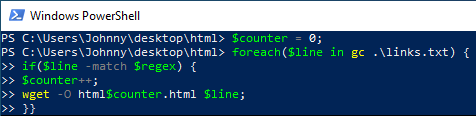
\includegraphics[trim=0 0 0 0, clip, width=\textwidth] {ps-script.png}
    \caption{Script used to download the contents of 1000 unique URIs}
    \label{fig:ps-script}
\end{figure}

I used a single Python code to answer questions 1, 2, and 4, so I will include the code at the end of the file and reference it in each question. The tool I used to remove the HTML markup was BeautifulSoup.

\subsection*{Discussion}
The script was nearly identical to the script I used in HW 2, but I broke it up into multiple lines this time and used wget. There were a few errors, and whenever there was an error it caused me to be missing a file (for example, file number 160 is missing from the 1000 files). I included screenshots of the errors in the GitHub repo.

For removing HTML markup, I attempted to use boilerpipe, but there was an error involving JVC versions not matching with Python versions or something like that. I wasn't able to resolve the error, so then I attempted to use Goose. Goose had an option for either `url' or `raw\_html' for the argument. Since I was using files instead of urls, I tried the raw\_html argument, but the file outputs were all blank. I was also unable to resolve that issue, so I just defaulted back to BeautifulSoup. Unfortunately, BeautifulSoup had issues with reading about one-third of the files because of special characters, so I just discarded those files and moved on.

In the Python code at the end of the file, lines 14-18 show how I created soup objects and converted them into text. I kept trying to run the code and ended up with 3 different errors, so I made exeptions for each in lines 33-42, and printed the total number of documents that had errors on line 44. I don't remember the number, but I believe it was in the mid 300s. In lines 31-32, I created a new file for the cleaned version of the html, wrote the contents of the soup object, and then closed the file. The rest of the code (besides line 1) pertains to question 2.

\section*{QUESTION 2 - Rank with TF-IDF}
Choose a query term (e.g., ``coronavirus'') that is not a stop word (e.g, ``the''), not super-general (e.g., ``web''), and not HTML markup (e.g., ``http'') that is found in at least 10 of your documents. (Hint: you can use the Unix command grep -c on the processed files to identify a good query.) If the term is present in more than 10 documents, choose any 10 English-language documents from different domains from the result set. (If you do not end up with a list of 10 URIs, you've done something wrong.)

As per the example in the Module 06 slides, compute TF-IDF values for the query term in each of the 10 documents and create a table with the TF, IDF, and TF-IDF values, as well as the corresponding URIs. (If you are using LaTeX, you should create a LaTeX table. If you are using Markdown, view the source of this file for an example of how to generate a table.) Rank the URIs in decreasing order by TF-IDF values.

You can use Google or Bing for the DF estimation. If you use Google, use 55 B as the total size of the corpus, and if you use Bing, use 12 B as the total size of the corpus (based on data from \url{https://www.worldwidewebsize.com}).

Don't forget the log base 2 for IDF, and mind your significant digits!

\subsection*{Answer}
\subsection*{TF-IDF Rankings}
\begin{center}
\begin{tabular}{ |c|c|c|c|c| } 
 \hline
 \textbf{File Number} & \textbf{TF-IDF} & \textbf{TF} & \textbf{IDF} & \textbf{URL}\\
 \hline
 210 & 0.00485 & 0.000788 & 6.149 & \url{https://www.cbc.ca}\\
 123 & 0.00480 & 0.000781 & 6.149 & \url{http://www.msn.com}\\
 67 & 0.00392 & 0.000637 & 6.149 & \url{https://businessdesk.co.nz}\\
 109 & 0.00272 & 0.000442 & 6.149 & \url{https://apnews.com}\\
 44 & 0.00178 & 0.000289 & 6.149 & \url{https://www.foxnews.com}\\
 197 & 0.00155 & 0.000252 & 6.149 & \url{https://www.theatlantic.com}\\
 7 & 0.00139 & 0.000227 & 6.149 & \url{https://www.nytimes.com}\\
 27 & 0.000704 & 0.000114 & 6.149 & \url{https://www.thedailybeast.com}\\
 199 & 0.000469 & 0.0000764 & 6.149 & \url{https://www.theguardian.com}\\
 116 & 0.000423 & 0.0000688 & 6.149 & \url{https://www.chicagotribune.com}\\
 \hline
\end{tabular}
\end{center}

\subsection*{Full URLs}
\begin{itemize}
    \item \url{https://www.cbc.ca/news/health/coronavirus-risk-canada-weather-1.5930135}
    \item \url{http://www.msn.com/en-us/weather/newspolitics/house-passes-bidens-new-dollar19-trillion-coronavirus-economic-relief-bill/vi-BB1e4ZCB?ocid=st}
    \item \url{https://businessdesk.co.nz/article/coronavirus/activate-money-where-and-how-to-get-lockdown-support-payments}
    \item \url{https://apnews.com/article/gretchen-whitmer-michigan-indictments-coronavirus-pandemic-traverse-city-10f7e02c57004da9843f89650edd4510}
    \item \url{https://www.foxnews.com/us/states-reopen-roll-back-mask-mandates-coronavirus}
    \item \url{https://www.theatlantic.com/politics/archive/2020/11/trumps-lies-about-coronavirus/608647/}
    \item \url{https://www.nytimes.com/2021/02/27/us/politics/coronavirus-vaccine-refusal-military.html?smid=tw-share}
    \item \url{https://www.thedailybeast.com/fda-issues-emergency-use-authorization-for-johnson-and-johnson-coronavirus-vaccine?source=twitter&via=mobile}
    \item \url{https://www.theguardian.com/us-news/live/2021/feb/22/joe-biden-coronavirus-covid-white-house-texas-donald-trump-live-updates?CMP=share_btn_tw}
    \item \url{https://www.chicagotribune.com/coronavirus/ct-re-couples-neighbors-covid-building-tt-20210223-eae4bavifvhijcc2q3wjeqt7pa-story.html}
\end{itemize}

\subsection*{Discussion}
I chose ``Virginia'' (case-sensitive) as my search term. To find the 10 unique URLs, I simply changed the tolerance level to 50 on line 21 to read ``if countTo10 < 50'' so that it would do the first 50 occurrences rather than the specific 10 numbers that I hardcoded into line 11. I then inspected each file number that was returned by hand until I found 10 unique domains that didn't show empty files. I did have an issue where the soup object would successfully read in data but then it would just write a blank file, so I had to just manually avoid those cases. It seems like that would happen whenever there were videos on the webpage, but I'm not sure. After I found the 10 unique files, I went back in and updated line 11 and line 21 to reflect those specific file numbers.

To calculate tf, idf, and tf-idf for each of the 10 links, I started by creating lists of size 10 in lines 8-10. I searched for ``Virginia'' on Google and got 775 million results, so I made a constant for that on line 12. You can ignore the ``keyCounter'' variable on line 6, as the only purpose of that was to see how many files had my keyword in it. I tried many different keywords until I found a suitable one this way. The important part starts on line 21 where I checked to see if I was currently iterating through one of my predetermined file numbers, then calculated the idf value on line 22 using 55 billion as the total size of Google and the constant from line 12 as the denominator, then calculated the tf value on line 28 by using the ``count()'' string method to count the number of instances of the keyword in the file and dividing that by a number that I manually input into the program (see next paragraph for more explanation), and finally calculated the tf-idf value near the end of line 48 where I output the results to the terminal by simply multiplying the tf and idf values from earlier. Lines 23-27 were purely for the sake of retrieving the URL to include in the above table.

To find each of the 10 counts for the number of instances of the keyword in each file, I ran a separate command in PowerShell using the ``Measure-Object'' command. Figure \ref{fig:ps-queries} shows my results.

\begin{figure}[h!]
    \centering
    % trim and clip are used to crop the image, trim=left bottom right top
    % width sets max width, height will be scaled appropriately
    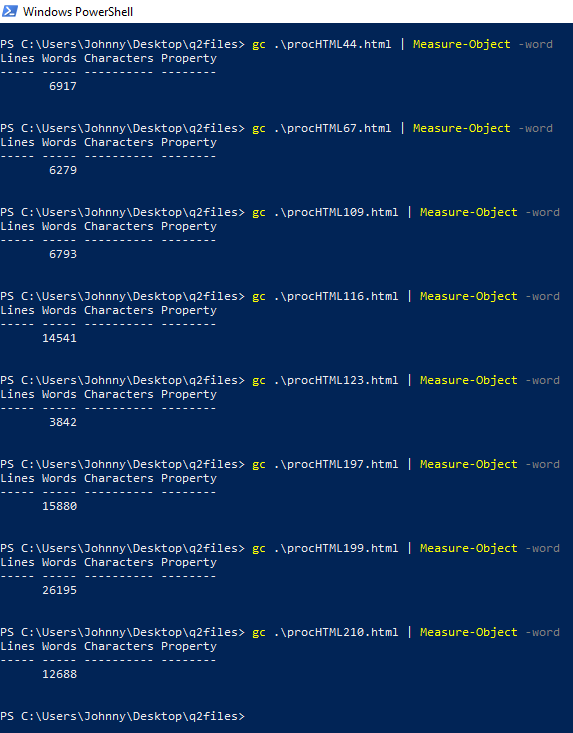
\includegraphics[trim=0 0 0 0, clip, width=\textwidth] {ps-queries.png}
    \caption{Commands used to count the number of instances of the keyword in each html file}
    \label{fig:ps-queries}
\end{figure}

\newpage
\section*{QUESTION 3 - Rank with PageRank}
Now rank the domains of those 10 URIs from Q2 by their PageRank. Use any of the free PR estimators on the web, such as:

\begin{itemize}
    \item \url{http://www.prchecker.info/check_page_rank.php}
    \item \url{http://www.checkpagerank.net/}
    \item \url{https://dnschecker.org/pagerank.php}
    \item \url{https://smallseotools.com/google-pagerank-checker/}
\end{itemize}

Note that these work best on domains, not full URIs.

If you use these tools, you'll have to do so by hand (they have anti-bot captchas), but there are only 10 to do.

Normalize the values they give you to be from 0 to 1.0. Use the same tool on all 10 (again, consistency is more important than accuracy).

Create a table similar to Table 1.

Briefly compare and contrast the rankings produced in Q2 and Q3.

\subsection*{Answer}
\subsection*{PageRank Rankings}
\begin{center}
\begin{tabular}{ |c|c|c|c|c| } 
 \hline
 \textbf{PageRank} & \textbf{Normalized PR} & \textbf{URL}\\
 \hline
 8 & 1.000 & \url{https://www.cbc.ca}\\
 8 & 1.000 & \url{http://www.msn.com}\\
 8 & 1.000 & \url{https://www.foxnews.com}\\
 8 & 1.000 & \url{https://www.theatlantic.com}\\
 8 & 1.000 & \url{https://www.thedailybeast.com}\\
 8 & 1.000 & \url{https://www.chicagotribune.com}\\
 7 & 0.875 & \url{https://www.theguardian.com}\\
 0 & 0.000 & \url{https://businessdesk.co.nz}\\
 0 & 0.000 & \url{https://apnews.com}\\
 0 & 0.000 & \url{https://www.nytimes.com}\\
 \hline
\end{tabular}
\end{center}

\subsection*{Discussion}
I used prchecker to rank the 10 URIs. It gave me a ranking from 1 to 10. It was unfortunate that all but 1 of them were either tied for first at 8 or tied for last at 0, so it didn't really give a good picture of how these websites compare. Aside from that, though, the rankings mirrored the rankings from table 1 fairly well with the exception of the ones that were ranked 0. I'm guessing those are just not ranked at all, and if they were ranked then they would be higher than 0 and match table 1 much more closely. The one thing that I would say is not very close between the 2 tables is the fact that in table 1, most of the rankings were not that close to each other, whereas in table 2, the top 6 URLs were ranked equally.

\section*{QUESTION 4 - Extra Credit (2 points)}
Re-do Q2 using the documents you collected in Q1 as the corpus instead of all of the Web. You should have 1000 total documents collected from Twitter, and you can use grep to discover how many of those documents contain your query term. Compare this ranking to those obtained in Q2 and discuss.

\subsection*{Answer}
If I had more time to finish typing this up and submitting it, I could easily just use the keyCounter variable from line 20 to do these calculations, but unfortunately the assignment is due in 30 minutes. I have quit one of my jobs, so after HW 4 I should be able to stay ahead of the assignments better!

\section*{References}
No references were used for this assignment.

\newpage
\lstinputlisting[language=Python, caption=Python code to collect 1000 unique links from tweets, label=lst:import]{CleanHTML.py}

\end{document}